\documentclass[11pt]{article}

\usepackage[margin=1in]{geometry}
\usepackage{graphicx}
\usepackage{booktabs}
\usepackage{amsmath}
\usepackage{amssymb}
\usepackage{hyperref}
\usepackage{xcolor}
\usepackage{tikz}
\usetikzlibrary{arrows.meta, positioning, calc, fit}

\title{\textbf{zklora: Verifiable Multi-Party Inference for Evaluating Private LoRA Weights}}
\author{Anonymous Authors}
\date{\today}

\begin{document}

\maketitle

\begin{abstract}
In decentralized computing environments, one party may wish to fine-tune a publicly available base model with Low-Rank Adaptation (LoRA) but keep those adapter weights private, while another party wants to evaluate performance on new data. 
We introduce \texttt{zklora}, a library designed to help the \emph{Base Model User} \emph{verifiably assess} the quality of a private LoRA module for a target task---for instance, to run a validation experiment without directly accessing the private weights. 
By adopting a multi-party inference approach and generating \emph{verifiable computations}, \texttt{zklora} enables the \emph{Base Model User} to confirm that remote LoRA computations are correct, all without seeing the private weights themselves. 
We demonstrate the feasibility of \texttt{zklora} via benchmark experiments, showing that our approach remains computationally viable across various model sizes, with notably fast verification times.
\end{abstract}

%------------------------------------------
% 1. PRELIMINARY RESULTS
%------------------------------------------
\section{Preliminary Results}

We benchmarked \texttt{zklora} by measuring the creation and verification times for our verifiable computations across multiple base models and private LoRA configurations. For each model, we computed a forward pass for a batch of 3 items with sequence length 5. 
Each experiment simulates the workflow where the \emph{Base Model User} uses local data to evaluate the base model + LoRA combination, requesting remote LoRA computations from the \emph{LoRA Owner}. 
We report total and average proof-generation times (\texttt{total\_prove}, \texttt{avg\_prove}) and verification times (\texttt{total\_verify}, \texttt{avg\_verify}), as well as relevant model parameters.

\begin{table}[ht]
    \centering
    \small
    \begin{tabular}{l c c c c c c c}
    \toprule
    \textbf{base\_model} & \textbf{\#lora} & \textbf{total\_params} & \textbf{avg\_params} & \textbf{total\_prove} & \textbf{avg\_prove} & \textbf{total\_verify} & \textbf{avg\_verify} \\
    \midrule
distilgpt2 & 24 & 589824 & 24576.0 & 759.33 & 31.64 & 16.56 & 0.69 \\
gpt2 & 48 & 2359296 & 49152.0 & 1675.58 & 34.91 & 32.79 & 0.68 \\
Llama-3.2-1B & 32 & 851968 & 26624.0 & 991.93 & 31.00 & 24.91 & 0.78 \\
Llama-3.3-70B-Instr. & 80 & 11796480 & 147456.0 & 3749.76 & 46.87 & 123.11 & 1.54 \\
Llama-3.1-8B-Instr. & 32 & 5242880 & 163840.0 & 1527.40 & 47.73 & 35.79 & 1.12 \\
Mixtral-8x7B-Instr. & 32 & 10485760 & 327680.0 & 2357.61 & 73.68 & 44.30 & 1.38 \\
    \bottomrule
    \end{tabular}
    \caption{Benchmark results for \texttt{zklora} showing multi-party inference overhead on various model + LoRA combinations. Times are in seconds.}
    \label{tab:results}
\end{table}

Notably, although proof-generation times can grow with model size, verification remains comparatively fast (e.g., \texttt{avg\_verify} of about 1--2 seconds even for 70B-scale models). This result demonstrates that \texttt{zklora} allows frequent correctness checks without excessive overhead, which is crucial for real-world “trial runs.” In larger-scale usage scenarios, once trust in the LoRA module is established, \texttt{zklora} may no longer be needed.

%------------------------------------------
% 2. MULTI-PARTY INFERENCE METHOD
%------------------------------------------
\section{Multi-Party Inference: zklora for Verifiable Evaluation}
Our aim is to enable the \emph{Base Model User} to run a \emph{validation experiment} on their local data, incorporating the private LoRA module from the \emph{LoRA Owner}. The Base Model User can measure task performance (e.g., cross-entropy loss, accuracy) to decide whether the LoRA meets performance requirements. 

Figure~\ref{fig:toy-mlp-lora} illustrates a simple scenario:
\begin{enumerate}
    \item \textbf{Base Model Forward Pass (Base Model User).}
    The \emph{Base Model User} runs layers without LoRA parameters locally, generating partial activations.

    \item \textbf{Forward to LoRA Adapter (Base Model User).}
    Whenever the next layer includes a LoRA transform, the \emph{Base Model User} sends these partial activations to the \emph{LoRA Owner}, who holds the private LoRA module.

    \item \textbf{LoRA Computation \& Proof Generation (LoRA Owner).}
    The \emph{LoRA Owner} applies the LoRA transformation to the activations and returns the updated activations alongside a \emph{cryptographic proof} of correctness. In our setup, \texttt{zklora} interfaces with \texttt{ezkl} to produce these proofs.

    \item \textbf{Resuming the Forward Pass (Base Model User).}
    The \emph{Base Model User} injects the updated activations back into the local model state and continues the forward pass. 

    \item \textbf{Verification \& Validation (Base Model User).}
    The \emph{Base Model User} verifies the LoRA proof. If valid, the outputs from the combined base + LoRA model are guaranteed to match the LoRA Owner’s claimed computation. The Base Model User can now measure final metrics (loss, accuracy, etc.) to assess \emph{quality} on the target task.
\end{enumerate}

\begin{figure}[ht]
\centering
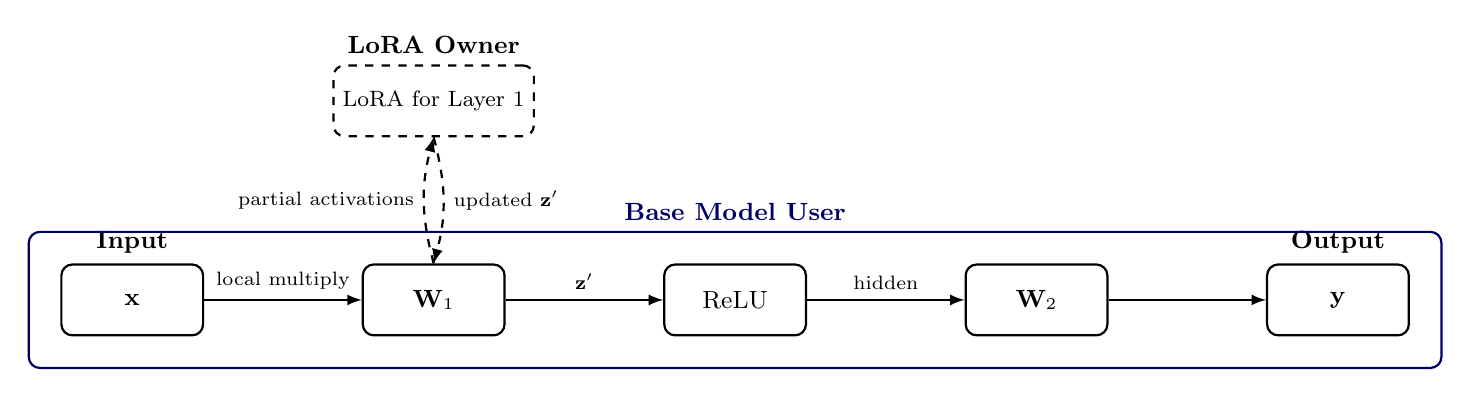
\begin{tikzpicture}[
    font=\small,
    >=latex,
    thick,
    block/.style={
      draw,
      rounded corners,
      align=center,
      minimum width=1.8cm,
      minimum height=0.9cm
    },
    dashedblock/.style={
      draw,
      dashed,
      rounded corners,
      align=center,
      font=\footnotesize,
      fill=white,
      minimum width=1.8cm,
      minimum height=0.9cm
    },
    arrow/.style={->, thick},
    node distance=2.0cm
]

\node[block, label=above:\textbf{Input}] (input) {$\mathbf{x}$};
\node[block, right=2.0cm of input] (W1) {$\mathbf{W}_1$};
\node[dashedblock, above=1.6cm of W1, label=above:\textbf{LoRA Owner}] (LoRA) {LoRA for Layer 1};
\node[block, right=2.0cm of W1] (act) {ReLU};
\node[block, right=2.0cm of act] (W2) {$\mathbf{W}_2$};
\node[block, label=above:\textbf{Output}, right=2.0cm of W2] (output) {$\mathbf{y}$};

\draw[->] (input) -- node[above, font=\scriptsize]{local multiply} (W1);
\draw[->, dashed] (W1.north) to[bend left=15] node[left, font=\scriptsize]{partial activations} (LoRA.south);
\draw[->, dashed] (LoRA.south) to[bend left=15] node[right, font=\scriptsize]{updated $\mathbf{z}'$} (W1.north);
\draw[->] (W1) -- node[above, font=\scriptsize]{$\mathbf{z}'$} (act);
\draw[->] (act) -- node[above, font=\scriptsize]{hidden} (W2);
\draw[->] (W2) -- (output);

\node[draw, rounded corners, thick, color=blue!40!black,
      fit=(input)(W1)(act)(W2)(output),
      label={[font=\small, color=blue!40!black]above:\textbf{Base Model User}},
      inner sep=0.4cm
] (baseModelFit) {};
\end{tikzpicture}
\caption{A simplified 2-layer MLP with LoRA on the first layer. The Base Model User (blue box) runs most computations locally but calls the LoRA Owner (dashed box) to update partial activations. After verifying correctness, the Base Model User can measure final metrics to decide whether to adopt the private LoRA more extensively.}
\label{fig:toy-mlp-lora}
\end{figure}

%------------------------------------------
% 3. INTRODUCTION
%------------------------------------------
\section{Introduction}
Large Language Models (LLMs) excel at a variety of tasks but come with significant computational and storage costs \cite{brown2020language, devlin2018bert}. 
Low-Rank Adaptation (LoRA) \cite{hu2021lora} addresses these costs by introducing a small number of trainable parameters into the model, drastically reducing memory overhead for fine-tuning \cite{ding2022delta}. 

When two entities, a \emph{LoRA Owner} and a \emph{Base Model User}, collaborate on a shared LLM, they may have conflicting constraints. The \emph{LoRA Owner} wants to keep custom LoRA weights private (e.g., for competitive or regulatory reasons), while the \emph{Base Model User} wants to \emph{test} or \emph{validate} these LoRA weights on a target task before deciding whether to deploy them at scale. Under normal circumstances, either the LoRA must be fully shared (sacrificing privacy), or the Base Model User must trust the LoRA Owner’s claims about performance with little evidence.

In this paper, we present \texttt{zklora}, a library that provides a \emph{verifiable computation} solution for the \emph{Base Model User} to \emph{evaluate} a private LoRA module. By orchestrating a multi-party inference, \texttt{zklora} allows the Base Model User to run the base model locally while sending partial activations to the LoRA Owner. Crucially, the LoRA Owner returns not only updated activations but also a cryptographic \emph{proof} that the correct LoRA transformation was applied. In this way, the Base Model User can confirm the final outputs truly reflect the LoRA module’s capabilities. After verifying and measuring results on a validation dataset, the Base Model User can later choose how to adopt the LoRA at larger scale.

%------------------------------------------
% 4. RELATED WORK
%------------------------------------------
\section{Related Work}

\subsection{Low-Rank Adaptation}
LoRA \cite{hu2021lora} has emerged as a popular way to efficiently fine-tune LLMs by injecting small, low-rank matrices into specific layers. This approach scales well, requiring less GPU memory than full fine-tuning. Various frameworks build on LoRA for GPT-2, GPT-Neo, LLaMA, and others \cite{ding2022delta}. By confining most updated parameters to low-rank adapter matrices, LoRA drastically reduces memory overhead during fine-tuning. As a result, domain-specific LoRA modules can be swapped in or out of the same base model, avoiding the need to retrain or store complete copies of large networks.

\subsection{Incrementally Verifiable Computation}
Valiant~\cite{valiant2008incrementally} introduced the notion of Incrementally Verifiable Computation (IVC), which offers updatable, compact proofs of correctness over multi-step computations. Nova~\cite{kothapalli2022nova} and HyperNova~\cite{kothapalli2024hypernova} refine these ideas, leveraging folding schemes and zero-knowledge properties to enable scaling of verifiable computations in multi-step neural network inference. IVC-based approaches align well with repeated computations needing multiple checkpoints of trust, such as multiple forward passes or partial training loops.

%------------------------------------------
% 5. CONCLUSION
%------------------------------------------
\section{Conclusion}
\texttt{zklora} enables a \emph{Base Model User} to verify the quality of a private LoRA module without revealing the LoRA weights. By pairing multi-party inference with cryptographic proofs, \texttt{zklora} ensures that the user can trust the computed outputs during validation experiments. After verifying performance, the Base Model User may adopt any approach they choose to integrate or deploy the private LoRA more widely, since the module has been proven effective. Our experiments show this approach is feasible across a range of model sizes, with \emph{fast verification times} minimizing the overhead of a verifiable evaluation phase. Future directions include further circuit optimization and exploring multi-owner scenarios, in which multiple private LoRA modules could be composed and verified within the same pipeline.

\bibliographystyle{plain}
\bibliography{references}

\end{document}
